\section{Scale-Out Streaming and Deployment Evidence}

The largest reported operational gains appear when the model keeps revisiting
nearly the same visual state. We treat the Gemma 4 26B streaming stack as a
scale-out lane for the same anti-recomputation questions, not as decorative
application color. The current draft still labels those rows separately because
they use a different model, machine, runtime, and streaming protocol; promoting
them to first-class evidence requires the same artifact-compatible outputs and
matched baselines used by the local experiments. Under the current protocol,
the stack reports 0.8\,s median same-video follow-up latency at 10--18$\times$
speedup, paired Streaming VideoMME results with 13$\times$ fewer ViT calls and
\mbox{$\sim$50$\times$} less dominant measured subpipeline compute, and selected
real-video regimes with 4.2--4.5$\times$ end-to-end speedups. ``Dominant
measured subpipeline'' is the instrumented high-cost streaming segment in that
runtime, not a full end-to-end denominator. Reported live-camera measurements
show the same regime dependence in the wild: one post-fix RTSP demo reduces
ViT calls by 14.3$\times$ over an active 60\,s window, while broader
scene-dependent 5--300$\times$ live-counter ranges remain appendix-weighted
until matched baselines land.

These rows are not local headline cells yet. They are included because they
show the scale of the operational regime where a stable scene is queried
repeatedly. The right current claim is that the scale-out lane exercises the
same anti-recomputation structure under a native streaming workload, not that
its counters can be multiplied into the local C-VISION or C-PERSIST numbers.
The paper-facing goal is to turn this lane into a first-class
\emph{streaming state reuse} evaluation with the same paired outputs, cache
correctness smoke tests, low-FPS / screenshot-polling / recency baselines, and
artifact bundle as the controlled local runs.

Smaller-$N$ UI studies stay strictly illustrative, not headline-bearing. The
sectional-scroll case studies remain explicitly weaker than the paired
streaming and real-video measurements above, and the contact-sheet imagery
below is qualitative rather than quantitative. The main-body evidence for this
section is the deployment table below.

\begin{table}[H]
\centering
\caption{Heterogeneous operational evidence for the streaming/deployment
regime. Metric type is shown explicitly because these rows mix component
counters, end-to-end timing, and live observations with different sample sizes
and denominators. Smaller UI and demo case studies are discussed in text and
kept clearly weaker than the paired streaming rows below. All scale-out rows are
pending artifact harmonization before they become first-class evidence in the
same claim graph as the local runs.}
\label{tab:real-apps}
\footnotesize
\renewcommand{\arraystretch}{1.16}
\begin{tabularx}{\linewidth}{@{}
  >{\raggedright\arraybackslash}p{0.18\linewidth}
  >{\raggedright\arraybackslash}p{0.16\linewidth}
  >{\raggedright\arraybackslash}X
  >{\raggedright\arraybackslash}p{0.16\linewidth}
@{}}
\toprule
Setting & Metric type & Outcome & Evidence class \\
\midrule
Streaming VideoMME (Gemma 26B) & component counter + accuracy & reported paired N=60: 13$\times$ fewer ViT calls; $\sim$50$\times$ less dominant measured subpipeline compute in the instrumented streaming segment; 58.3/60.0/61.7\% (stream/token-prune/dense), all within the reported $\pm$12 pp 95\% CI & scale-out stream benchmark \\
Real-video paired regimes (Gemma 26B) & end-to-end timing & reported 4.2--4.5$\times$ end-to-end speedup on talking-head and surveillance-style real-video measurements & scale-out real-video benchmark \\
Gemma 26B same-video follow-up & follow-up latency & reported N=20 VideoMME follow-up subset: 0.8\,s median follow-up; 10--18$\times$ faster than cold prefill; aggregate accuracy 65.0\% with and without KV reuse & scale-out follow-up benchmark \\
Live-camera pipeline & live component counter & reported single-system counter: 14.3$\times$ fewer ViT calls on one active 60\,s RTSP window (701 decoded frames / 49 ViT calls); broader 5--300$\times$ scene-dependent range remains appendix-weighted live-counter evidence & scale-out live measurement \\
\bottomrule
\end{tabularx}
\end{table}

The Qwen composition experiments do not yet reproduce this operational story as
a fidelity-preserving stack. The original stacked run reproduced the speedup
side but failed the accuracy budget. The dense-first-query admission successor
restores first-query aggregate correctness and leaves a follow-up-only
near-miss, but it also shows why the claim boundary must stay strict. The
long-bucket continuations now measure follow-up image-token activity directly
and find none: all follow-up image tokens are cache-served under the current
prompt-cache path, and every tested long-Q0 keep rate misses the target
fidelity/speed band.
That lane is therefore dense-first-query admission plus K-cache reuse rather
than proof of active follow-up vision pruning. That is why
Table~\ref{tab:real-apps} is operational evidence rather than part of the local
C-VISION or C-PERSIST headline rows.

\begin{figure}[H]
  \centering
  \IfFileExists{generated/figures/streaming_snapshot_contact_sheet.png}{
    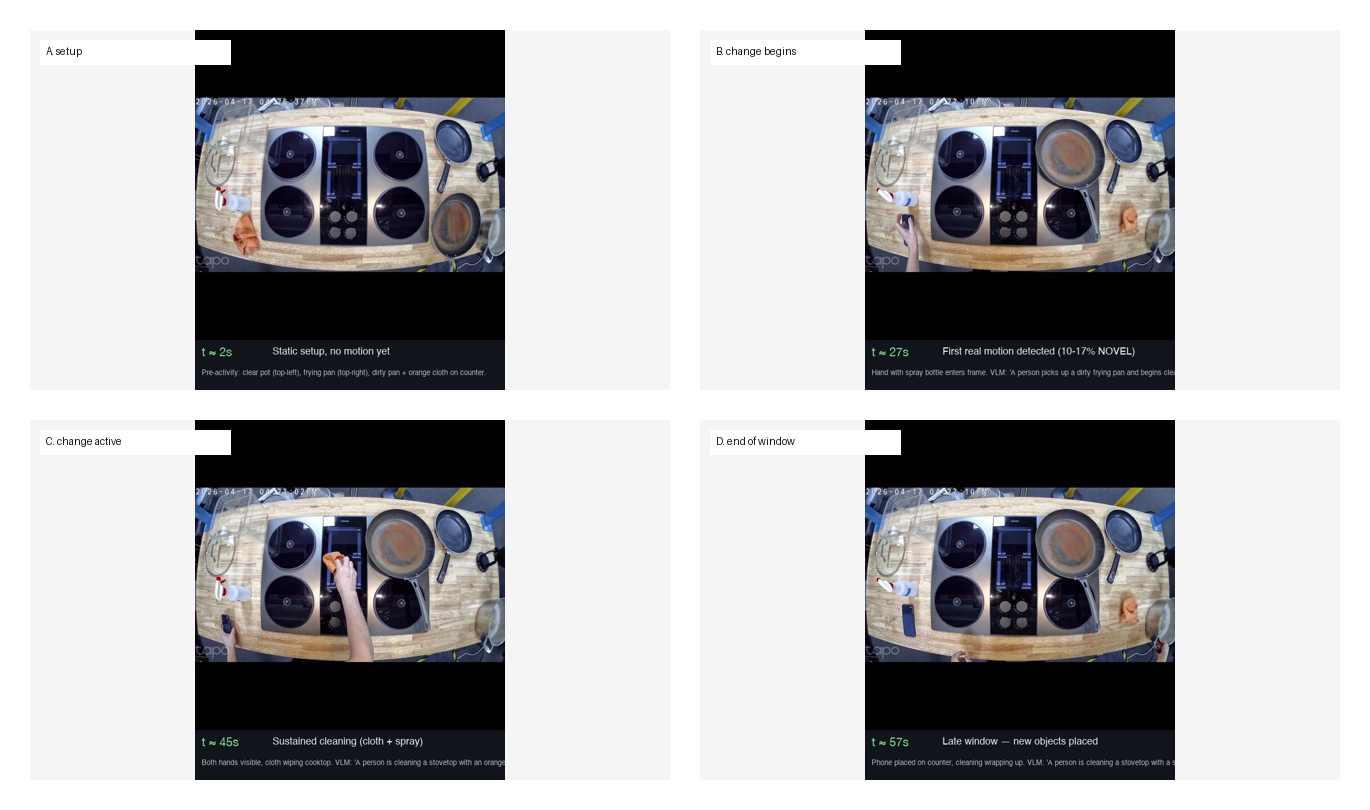
\includegraphics[width=\linewidth]{generated/figures/streaming_snapshot_contact_sheet.png}
  }{
    \fbox{\parbox{0.9\linewidth}{Run \texttt{make paper-sync} to generate the streaming/UI contact sheet or a placeholder.}}
  }
  \caption{Representative imagery from the post-fix RTSP demo. These snapshots
  are qualitative only; they illustrate an active-scene live deployment, but
  the quantitative deployment claims in Table~\ref{tab:real-apps} come from the
  paired streaming, real-video, and live-camera measurements rather than from
  this contact sheet.}
  \label{fig:streaming-contact-sheet}
\end{figure}

The current streaming evidence does not yet close a full systems-reviewer
checklist. The paper still lacks the screenshot-polling baseline, low-FPS dense
baseline, SimpleStream-style recency baseline, broader UI diversity, and a
dedicated stale-cache failure case. The scale-out lane should next run the same
claim axes as the local paper: a cache-correctness smoke test, C-PERSIST
same-video follow-up replication, measured sparse-ViT / ceiling validation,
native streaming matched baselines, and a raw re-export of the large sparse
exactness artifact with item IDs, paired outputs, parse failures, and
confidence intervals. What it already suggests is that the same
anti-recomputation principle can appear outside sparse benchmark slices, in the
regime where users keep asking the same system about nearly the same scene.

\begin{sectiontodo}{Keep scale-out evidence reviewer-safe}
The next useful additions are a screenshot-polling baseline, a wider UI set,
and one concrete failure case where stale-cache decisions break trust. Keep the
section tied to the scale-out evidence above. Smaller UI claims such as
sectional scroll, threshold tuning, or affine-axis mechanism variants should
stay appendix-weighted until their evidence is cleaned up further.

\textcolor{todoBorder}{Remaining work: add cache-correctness smoke artifacts
for the 26B stack, a C-PERSIST scale-out replication, measured sparse-ViT /
ceiling validation, screenshot-polling and low-FPS dense baselines, broader UI
coverage, and one stale-cache failure case before making the streaming lane
carry more of the headline.}
\end{sectiontodo}
